
%================================================================
\chapter{Simulation-Based Inference}\label{chap:sbi}
%================================================================

Computational neuroscientists have developed complex mechanistic models to describe neural phenomena of interest. Many mechanistic models are defined through simulators which describe how the process generates data. However, simulators are poorly suited for inference and lead to challenging inverse problems. Standard Bayesian inference is performed within the context of a statistical model from which the likelihood can be derived. Likelihoods are generally intractable or computationally infeasible for simulator models, which makes the typical approach to inference inaccessible. 

In this chapter we discuss \textit{simulation-based inference} (SBI), that is, algorithms that avoid explicit likelihood evaluations by instead using model simulations. SBI is perhaps best known under the moniker \textit{likelihood-free inference} (LFI). Nevertheless, we prefer the term SBI to LFI as the latter indicates that the likelihood is not present at all, which we will see is not the case.

From this chapter and onwards, there will be a minor notational tweak. In order to avoid ambiguity, observed data will be denoted by $y_\mathrm{obs}$ and simulated data, generated by the simulator model, by $y_\mathrm{sim}$.


%=============================================================== 
\section{Likelihood-Based vs. Simulation-Based}
%=============================================================== 

In this section, we detail the differences between likelihood-based and simulation-based inference. The content of this section is based on \cite{abc_handbook}, \cite{sbi_review} and \cite{snl_thesis}.


Suppose a data-generating process is controlled by parameters $\theta$, and the process generates data $y$ when run forward. We assume that the process defines the conditional likelihood function $\lhood$ for every setting of $\theta$. Given an observation $y_\mathrm{obs}$, the problem of interest is to infer parameter settings compatible with $y_\mathrm{obs}$. That is, we want to compute the posterior density $\pi \qty(\theta \mid y_\mathrm{obs})$  obtained by Bayes' theorem (\autoref{eq:bayes_unnorm}). The choice of inference algorithm primarily depends on how the data-generating process is modelled. 

A purely statistical model, or an \textit{explicit model}, describes the likelihood $p \qty(y_\mathrm{obs} \mid \theta)$ of the process given values for $y_\mathrm{obs}$ and $\theta$. With an explicit model, the posterior $\pi \qty(\theta \mid y_\mathrm{obs})$ is, in general, easily evaluated using Bayes' theorem. Samples from the posterior can be generated using Bayesian computation methods such as Markov chain Monte Carlo algorithms, as discussed in \cref{sec:bayesian_computation}. Such methods are referred to as \textit{likelihood-based inference} methods, as they explicitly evaluate the likelihood.   

On the other hand, a \textit{simulator model}, or an \textit{implicit model}, describes how the process generates data. Many mechanistic models are defined through simulator models. For any parameter setting $\theta$, a simulator model can be run forward to generate samples from the likelihood $p \qty(y_\mathrm{obs} \mid \theta)$. Unlike for explicit models, implicit simulator models generally have intractable or computationally infeasible likelihoods. The complexity or absence of the associated likelihood typically arises from it involving computationally expensive or intractable integrals, or that the simulator's internal states are unavailable. In order to perform inference on a simulator model, methods using simulations from the model rather than likelihood evaluations are needed. Such methods are referred to as \textit{simulation-based inference} methods.

In general, simulation-based methods are less efficient than likelihood-based as the former can require lots of simulations to produce accurate results. One of the main topics of research in simulation-based inference is how to reduce the required number of simulations without sacrificing inference quality.


%================================================================
\section{Approximate Bayesian Computation}\label{sec:abc}
%================================================================ 

%Approximate Bayesian Computation (ABC) constitutes a class of computational algorithms rooted in Bayesian statistics that can be used to evaluate posterior distributions of model parameters without having to explicitly calculate likelihoods. ABC algorithms approximate the likelihood by assessing how likely it is the model could have produced the observed data. This is done by comparing simulated data, generated by the simulator, to the observed data. The simulations that do not reproduce the observed data within a distance specified by a tolerance are discarded. 

Approximate Bayesian Computation (ABC) constitutes a class of computational algorithms rooted in Bayesian statistics that can be used to evaluate posterior distributions of model parameters without having to explicitly calculate likelihoods. In this section we discuss ABC and its two fundamental algorithms: the original \textit{rejection ABC} algorithm and the more sophisticated \textit{Markov chain Monte Carlo (MCMC) ABC} algorithm. 

The content of this section is mainly based on material from \cite{abc_handbook}.

%=============================================================== 
\subsection{The ABC of Approximate Bayesian Computation}
%=============================================================== 

Given observed data $\yobs$, a simulator model $\mathrm{M}(\theta)$ with parameters $\theta$ having prior $\pi(\theta)$, we seek an algorithm to sample from the posterior $\pi \qty(\theta \mid \yobs) \propto p \qty(\yobs \mid \theta) \pi(\theta)$. This can be achieved by using the \textit{rejection sampling algorithm}: 

\begin{algorithm}[H]
\caption{Rejection sampler}
\label{alg:rej_sampler1}
\SetAlgoLined
\DontPrintSemicolon
 % Algorithm 
 \nl Sample $\theta \sim \pi (\theta)$.\;
 \nl Accept $\theta$ with probability proportional to the likelihood $p\qty(\yobs \mid \theta)$.\;
\end{algorithm}

\cref{alg:rej_sampler1} can be made more general and avoid the need to explicitly compute probabilities by using the following, stochastically equivalent, formulation: 

\begin{algorithm}[H]
\caption{General rejection sampler}
\label{alg:rej_sampler2}
\SetAlgoLined
\DontPrintSemicolon
 % Algorithm 
\nl Sample $\theta \sim \pi (\theta)$.\;
\nl Simulate data $\ysim$ from $\mathrm{M}(\theta)$.\;
\nl Accept $\theta$ if $\ysim = \yobs$.\;
\end{algorithm}

\cref{alg:rej_sampler2} is due to Rubin \cite{Rubin}. The chance of the outcome $\ysim = \yobs$ will, however, be vanishingly small for most problems, and thus vastly time consuming to compute. \cref{alg:rej_sampler2} will therefore, typically, not be an efficient algorithm. This is where the approximation to Bayesian computation comes into play. We define a discrepancy metric $\rho(\cdot, \cdot)$ to compare the simulated and observed data and a tolerance $\epsilon \geq 0$. The approximate Bayesian computation (ABC) algorithm is then: 

\begin{algorithm}[H]
\caption{Approximate rejection sampler}
\label{alg:rej_sampler3}
\SetAlgoLined
\DontPrintSemicolon
 % Algorithm 
 \nl Sample $\theta \sim \pi (\theta)$. \;
 \nl Simulate data $\ysim$ from $\mathrm{M}(\theta)$. \;
 \nl Compute $\rho \equiv \rho \qty(\ysim, \yobs)$, and accept $\theta$ as an approximate draw from $\pi \qty(\theta \mid \yobs)$ if $\rho \leq \epsilon$. \;
\end{algorithm}

\cref{alg:rej_sampler3} is called the \textit{rejection ABC algorithm} and was first proposed by Tavaré et al. in \cite{Tavare} and developed by Pritchard et al. in \cite{Pritchard}. In the scheme of Pritchard et al., the simulated and observed data were compared through a choice of summary statistics. We will discuss the algorithm in more detail in the next section. 


%=============================================================== 
\subsection{Rejection ABC}
%=============================================================== 

\textit{Rejection ABC}, as outlined in \cref{alg:rej_sampler3}, is a rejection sampling algorithm for obtaining independent samples from the approximate posterior $ \pi_\mathrm{ABC} \qty(\theta \mid \rho \qty(\ysim, \yobs) \leq \epsilon)$, where $\rho \qty(\cdot, \cdot)$ is a discrepancy metric, e.g. the Euclidean distance, and $\epsilon \geq 0$ a tolerance. The algorithm proceeds by first sampling a set of parameters $\theta$ from the prior, then generate simulated data $\ysim$ under the simulator model $\mathrm{M}\qty(\theta)$ specified by the sampled $\theta$, and finally accepting and retaining $\theta$ if the distance between $\ysim$ and $\yobs$ is no more than $\epsilon$. If $\rho \qty(\ysim, \yobs) = 0$, then $\ysim = \yobs$, and the accepted $\theta$ is a sample from the true posterior. The tolerance parameter $\epsilon$ thus controls the trade-off between estimation accuracy and computational efficiency. With sufficiently small $\epsilon$, the accepted samples follow the exact posterior more closely, though the algorithm accepts less often. On the other hand, the algorithm accepts more often with a large $\epsilon$, but the accepted samples might yield a replica of the prior.  

Stochastically matching $\ysim$ and $\yobs$ becomes increasingly difficult with increasing dimensionality of the data. In order to operate efficiently, ABC algorithms require a compression of the data into low-dimensional summary statistics $s = S(y)$. A summary statistic that contains the same amount of information about model parameters as the whole dataset, is referred to as being a sufficient statistic $\tilde{s}$. Thus, 

\begin{equation}
\begin{aligned}
    \pi \qty(\theta | \yobs ) &= \lim_{\epsilon \to 0} \pi_\mathrm{ABC} \qty(\theta \mid \rho \qty (\ysim, \yobs) \leq \epsilon) 
    \\
    &= \lim_{\epsilon \to 0} \pi_\mathrm{ABC} \qty(\theta \mid \rho \qty (\tilde{s}_\mathrm{sim}, \tilde{s}_\mathrm{obs}) \leq \epsilon)
    \\
    &\approx \lim_{\epsilon \to 0} \pi_\mathrm{ABC} \qty(\theta \mid \rho \qty (s_\mathrm{sim}, s_\mathrm{obs}) \leq \epsilon)
\end{aligned}
\end{equation}

The choice of summary statistics is crucial for the performance of ABC algorithms, and the optimal choice is a minimal sufficient summary statistic. It is common to use the Fisher-Neyman factorization theorem to determine whether or not a summary statistic is sufficient. The theorem is based on being able to re-express the likelihood as a function of the sufficient summary statistic and data. Unfortunately, in the context of simulation-based inference, the likelihood is unavailable and we cannot examine a summary statistic to determine if the Fisher-Neyman factorization theorem holds. However, if powerful low-dimensional summary statistics are established, ABC algorithms can still offer a reasonable performance. The dimension of the vector of summary statistics $s$ should be large enough so that it capture as many important features of the observed data as possible, but also low enough so the curse of dimensionality of matching $\ssim$ and $\sobs$ is avoided. 

\autoref{fig:abc_illustration} gives a conceptual overview of the rejection ABC algorithm in a two-dimensional summary statistic space. Having observed data $\yobs$ provided by nature and reduced it to a summary statistic $\sobs$ (the blue dot), we sample parameter values $\theta \sim \prior$, generate simulated data $\ysim$ through the simulator $\mathrm{M}(\theta)$, compute the simulated summary statistic $\ssim$ and compare with the observation. Here, the discrepancy metric is the Euclidean distance, and the acceptance region amounts to a circle (indicated by the shaded grey circle) with center according to the observation and radius determined by the tolerance $\epsilon$. The $\theta$'s that correspond to $\ssim$ within this circle are accepted (the green dots), and those outside the circle are rejected (the red dots). 

\begin{figure}[!htb]
    \centering 
    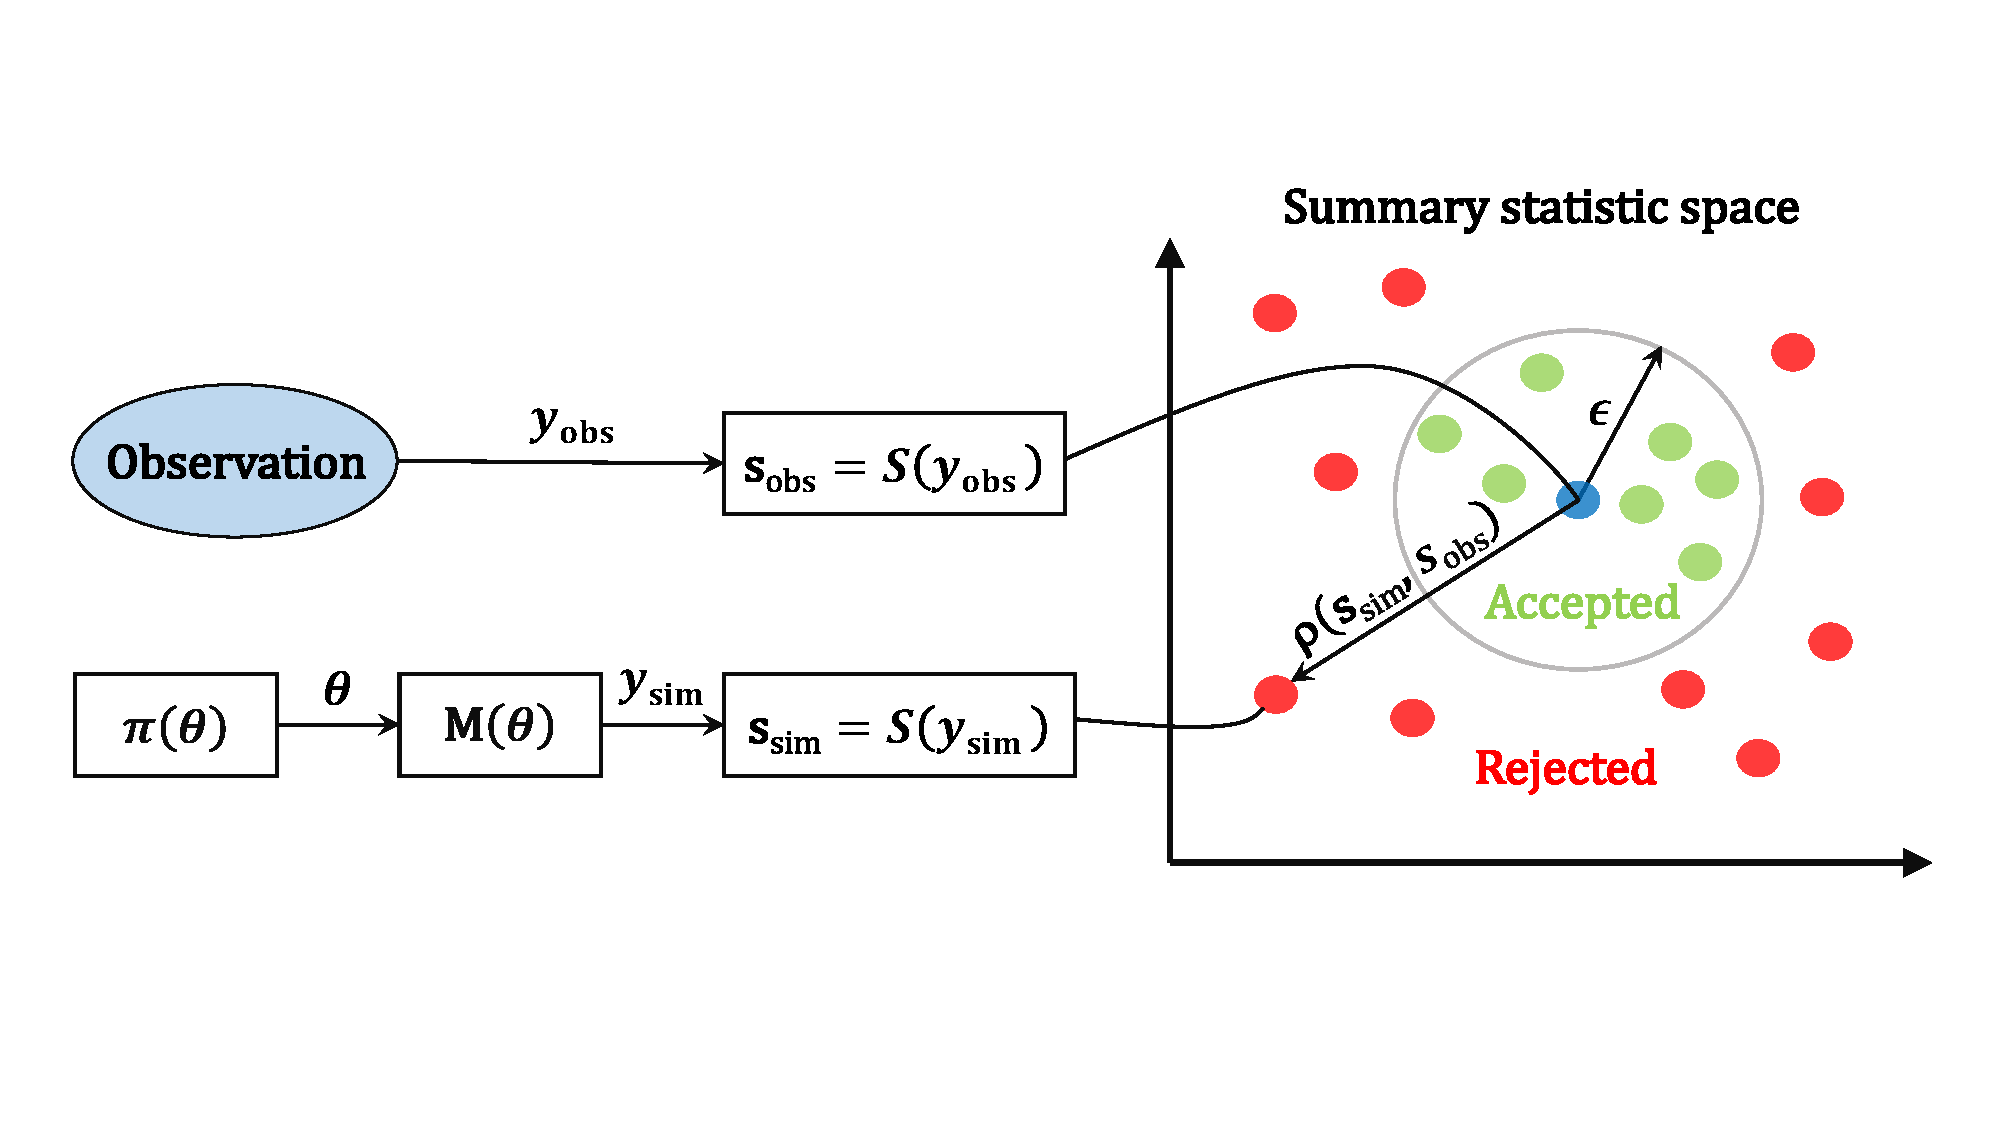
\includegraphics[scale=0.4]{ABC_illustration}
    \caption{A conceptual overview of rejection ABC in 2D summary statistic space. The discrepancy metric is the Euclidean distance, which has a circular acceptance region with the observed summary statistic $\sobs$ as center (blue dot) and tolerance $\epsilon$ as radius. The parameters $\theta$ with corresponding simulated summary statistics $\ssim$ that fall within the acceptance region are accepted (green dots), and those outside are rejected (red dots). See text for additional details.}
    \label{fig:abc_illustration}
    \source{Adapted from Fig. 3 in \cite{abc_figure}.}
\end{figure}

\cref{alg:rej_abc} summarizes the full rejection ABC algorithm.

\begin{algorithm}[H]
\caption{Rejection ABC}
\label{alg:rej_abc}
\SetAlgoLined
\DontPrintSemicolon
 % Algorithm 
 \textbf{Inputs\,:}\;
 \vspace{-5mm}
 \begin{itemize}
     \item An observation $\yobs$. 
     \item A simulator model $\mathrm{M}(\theta)$ with parameters $\theta$ having prior $\prior$.
     \item A discrepancy metric $\rho(\cdot, \cdot)$ and threshold $\epsilon \geq 0$. 
     \item A summary statistics function $S(y)$. 
     \item An integer $N>0$.
 \end{itemize}
 
 \vspace{5mm}
 \textbf{Sampling\,:}\;
 \For{$i=1, ..., N$}{ 
 \nl Sample $\theta \sim \prior$. \; 
 \nl Simulate data $\ysim $ from $M(\theta)$. \;
 \nl Calculate $\rho \equiv \rho \qty(S \qty(\ysim), S \qty(\yobs)) = \rho \qty(\ssim, \sobs)$. \; 
 \vspace{2mm}
 \eIf{$\rho \leq \epsilon$}{
   \nl Accept $\theta$. \;
   }{
   \nl Go to 1. \;
  }
 }
\end{algorithm}


%=============================================================== 
\subsection{Markov Chain Monte Carlo ABC}
%=============================================================== 

In Rejection ABC, the proposal parameters are sampled from the prior. Although sampling from the prior is efficient, the efficiency of the overall procedure will be determined by whether the prior is chosen so that it is of a similar shape and location as the desired posterior. The acceptance rate will be low if the approximate posterior is significantly narrower than the prior, as is often the case, and the rejection ABC algorithm will thus become more computationally inefficient as more of the expensive data generation becomes necessary. In this case, we might choose to develop a recursive strategy where the quality of previous candidates in our sampling algorithm can be used to guide the candidate generation process. Basing proposal samples off of previous states is precisely the strategy behind conventional Markov chain Monte Carlo (MCMC) methods, as we introduced in \cref{sec:bayesian_computation}. 

Beaumont et al. \cite{Beaumont} were the first to both extend the ABC approach to use MCMC methods and use the term \textit{Approximate Bayesian Computation}. \cref{alg:mcmcabc} summarizes the \textit{MCMC ABC} algorithm with Metropolis sampling (also discussed in \cref{sec:bayesian_computation}). To perform Metropolis sampling in the simulation-based context, we calculate the probability of accepting the proposal $\theta^*$ by evaluating: 

\begin{equation}\label{eq:abc_metropolis}
    \alpha = \begin{cases}
    \min \qty(1, \frac{\pi \qty(\theta^*)}{\pi \qty(\theta_{t-1})}) \qquad &\text{if } \rho \qty(\ssim, \sobs) \leq \epsilon 
    \\
    0 \qquad &\text{if } \rho \qty(\ssim, \sobs) > \epsilon 
    \end{cases}
\end{equation}

Similarly to rejection ABC, the acceptance probability of MCMC ABC decreases as $\epsilon$ becomes small. Moreover, the performance of MCMC ABC strongly depends on the selection of proposal and prior density. 

\begin{algorithm}[!htb]
\caption{Markov chain Monte Carlo ABC with Metropolis sampler}
\label{alg:mcmcabc}
\SetAlgoLined
\DontPrintSemicolon
 % Algorithm 
 \textbf{Inputs\,:}\;
 \vspace{-5mm}
 \begin{itemize}
    \item An observation $\yobs$. 
     \item A simulator model $\mathrm{M}(\theta)$ with parameters $\theta$ having prior $\prior$.
     \item A symmetric Markov proposal density $q \qty(\theta^* \mid \theta)$.
     \item A discrepancy metric $\rho(\cdot, \cdot)$ and threshold $\epsilon \geq 0$. 
     \item A summary statistics function $S(y)$. 
     \item An integer $N>0$.
 \end{itemize}
 
 \vspace{5mm}
 \textbf{Initialize\,:}\;
 \nl Sample $\theta_0$ by performing one iteration of rejection ABC (\cref{alg:rej_abc}).\;

 \vspace{5mm}
 \textbf{Sampling\,:}\;
 \For{$t=1, ..., N$}{ 
 \nl Generate proposal $\theta^* \sim q \qty(\theta^* \mid \theta_{t-1})$. \; 
 \nl Simulate data $\ysim $ from $M \qty(\theta^*)$. \;
 \nl Calculate $\rho \equiv \rho \qty(S \qty(\ysim), S \qty(\yobs)) = \rho \qty(\ssim, \sobs)$. \; 
 \nl Calculate acceptance criterion $\alpha$ (\autoref{eq:abc_metropolis}). \;
 \nl Sample $u \sim \mathrm{U}(0,1)$. \; 
 \vspace{2mm}
 \eIf{$u \leq \alpha$ and $\alpha \neq 0$}{
 \nl  $\theta_t = \theta^*$\;
   }{
  \nl $\theta_t = \theta_{t-1}$\;
  }
 }
\end{algorithm}

%=============================================================== 
\section{Regression Adjustment}
%=============================================================== 

should weight samples by distance from observation. 

In this section we discuss a post-sampling refinement called \textit{regression adjustment}. 


%=============================================================== 
\subsection{Linear Regression Adjustment}
%=============================================================== 



%=============================================================== 
\subsection{Local Linear Regression Adjustment}
%=============================================================== 



%===============================================================
\section{Neural Density Estimation}
%===============================================================


%===============================================================
\subsection{Sequential Neural Posterior Estimation}
%===============================================================

Sequential Neural Posterior Estimation (SNPE) is a novel algorithm for simulation-based inference. Dissecting all of the intricacies of SNPE is beyond the scope of this thesis. We will in this section provide an overview of the algorithm. For all details we refer the reader to the original articles \cite{SNL_first}, \cite{SNPE_first} and \cite{SNPE_apt}.

Sequential Neural Posterior Estimation (SNPE)\footnote{Source code available at \url{https://github.com/mackelab/delfi}} is a novel method for parameter inference. The method uses ABC to learn a neural network which maps features of observed data to the posterior distribution over parameters. The strategy was originally proposed by Papamakarios and Murray in \cite{papamakarios2016fast} and further developed by Lueckmann et al. in \cite{SNPE17} and \cite{SNPE19}. In the literature, the variant of Papamakarios and Murray is often referred to as SNPE-A and the variant of Lueckmann et al. as SNPE-B. In this essay, SNPE refer to the particular method by Lueckmann et al.

A \textit{conditional neural density estimator} is a parametric density model $q_{\bm{\phi}}$ (such as a neural network), where $\bm{\phi}$ are distribution parameters. With a pair of datapoints $(\bm{u}, \bm{v})$ as input, the model outputs a conditional probability density $q_{\bm{\phi}}(\bm{u}\mid \bm{v})$. Given a set of training data $\qty{\bm{u}_n, \bm{v}_n}_{1\colon N}$ that are independent and identically distributed according to a joint probability density $p(\bm{u}, \bm{v})$, $q_{\bm{\phi}}$ is trained by minimizing the loss $\mathcal{L} = - \sum_n \log q_{\bm{\phi}}(\bm{u}_n, \bm{v}_n)$ with respect to $\bm{\phi}$. With enough training data, and with a sufficiently flexible model, $q_{\bm{\phi}}(\bm{u}\mid \bm{v})$ will learn to approximate the conditional $p(\bm{u}\mid \bm{v})$ \cite{SNL18}. 

A neural density estimator $q_{\bm{\phi}}(\bm{\theta} \mid \bm{x})$ can be used to approximate the posterior $p \qty(\bm{\theta}\mid \bm{x}_0)$ as follows. First, a set of samples $\qty{\bm{\theta}_n , \bm{x}_n}_{1\colon N}$ is obtained from the joint distribution $p (\bm{\theta}, \bm{x})$, by $\bm{\theta}_n \sim \prior$ and $\bm{x}_n \sim p \qty(\bm{x} \mid \bm{\theta}_n)$ for $n=1, ..., N$. Then, $q_{\bm{\phi}}$ is trained using $\qty{\bm{\theta}_n , \bm{x}_n}_{1\colon N}$ as training data in order to a global approximation of $\posterior$. Finally, $p \qty(\bm{\theta} \mid \bm{x}_0)$ can be simply estimated by $q_{\bm{\phi}} \qty(\bm{\theta} \mid \bm{x}_0)$. In order to obtain an accurate posterior fit, this approach may require a large number of simulations to sample enough training data in the vicinity of $\bm{x}_0$ \cite{SNL18}. 

SNPE is a strategy for reducing the number of simulations needed by conditional neural estimation. Since simulations from parameters with low posterior density $p \qty(\bm{\theta} \mid \bm{x}_0)$ may not be useful in training $q_{\bm{\phi}}$, the key idea of SNPE is to generate parameter samples $\bm{\theta}_n$ from a proposal $\tilde{p}(\bm{\theta})$, that generates data $\bm{x}_n$ more likely to be in the vicinity of $\bm{x}_0$,  instead of the prior $\prior$ \cite{SNL18}. However, minimizing $\mathcal{L}$ on samples drawn from a proposal $\tilde{p}(\bm{\theta})$ no longer yields the target posterior but rather the \textit{proposal posterior}
\begin{equation}
    \tilde{p}(\bm{\theta} \mid \bm{x}) = p (\bm{\theta} \mid \bm{x}) \frac{\tilde{p}(\bm{\theta}) p(\bm{x}) }{\prior \tilde{p}(\bm{x}) },
\end{equation}
where $\tilde{p}(\bm{x}) = \int \tilde{p} (\bm{\theta}) \lhood d\bm{\theta}$ and it is assumed that $\tilde{p} (\bm{\theta})=0$ where $\prior = 0$ \cite{apt}. Hence, to account for sampling from a proposal $\tilde{p}(\bm{\theta})$, an adjustment of either the learned posterior or the proposed samples must be made. 

Lueckmann et al. deal with this problem by adjusting the parameter samples $\bm{\theta}_n$ by assigning them weights $w_n = p \qty(\bm{\theta}_n)/ \tilde{p} \qty(\bm{\theta}_n)$. During training SNPE minimizes an importance weighted loss $- \sum_n w_n \log q_{\bm{\phi}}(\bm{\theta}_n \mid \bm{x}_n)$, which allows for direct recovery of $p \qty(\bm{\theta} \mid \bm{x})$ from $q_{\bm{\phi}}$ with no correction and no restrictions on $p(\bm{\theta})$, $\tilde{p}(\bm{\theta})$ or $q_{\bm{\phi}}$ \cite{apt}. However, the weights can have a high variance, which can lead to slow or inaccurate inference \cite{SNL18}.
  
In \autoref{fig:snpe}, a conceptual overview of the SNPE method is shown.

\begin{figure}[H]
\begin{center}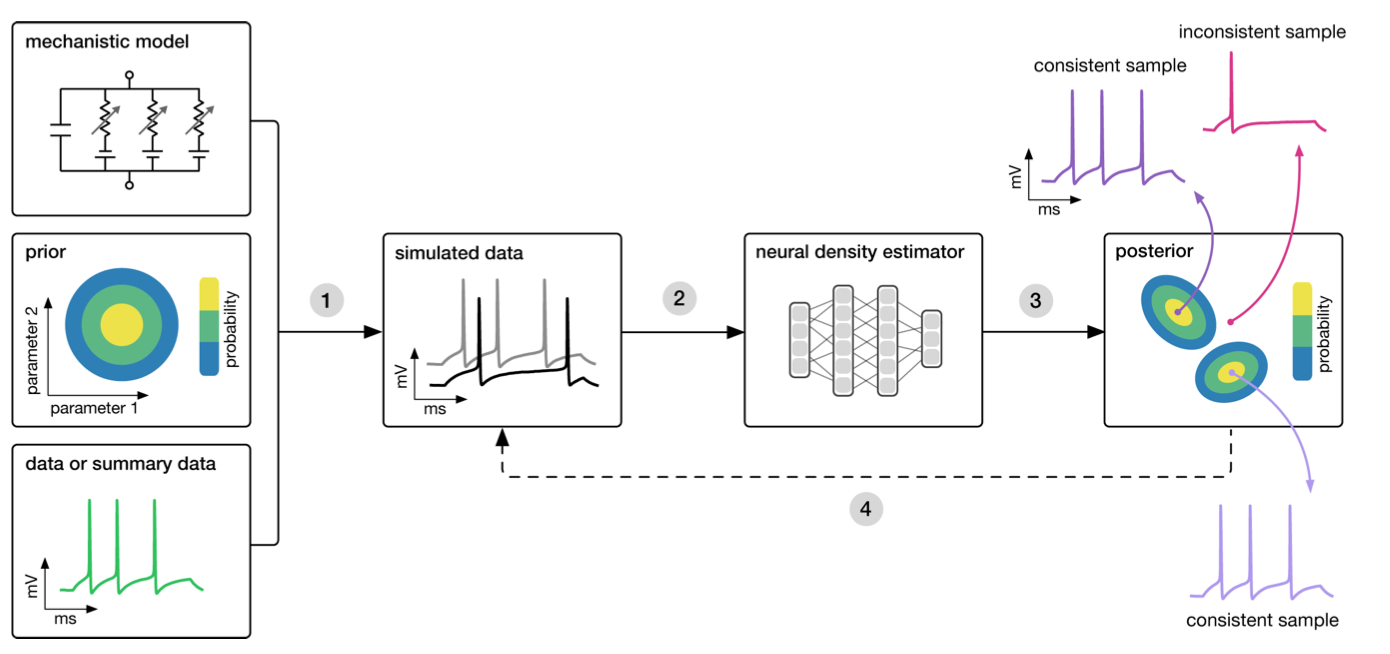
\includegraphics[scale=0.65]{snpe}
\end{center}
\caption{Parameter estimation by Sequential Neural Posterior Estimation (SNPE): a conceptual overview. Retrieved from \cite[Figure 1]{SNPE19}.}
\label{fig:snpe}
\end{figure}









    


